\section{Leitner's Learning Box Reviewed}

A \emph{Leitner's learning box}\footnote{http://en.wikipedia.org/wiki/Leitner\_system} is a simple but ingenious little contraption to support the tedious
process of memorization, especially prominent when trying to learn, for example, a new language that requires a lot of rote memorization.

% DETAILS HERE; REFER TO FIGURE BELOW TO EXPLAIN INCHING FORWARD, THEN FALLING ALL THE WAY BACK

\begin{figure}[htbp]
	\centering
  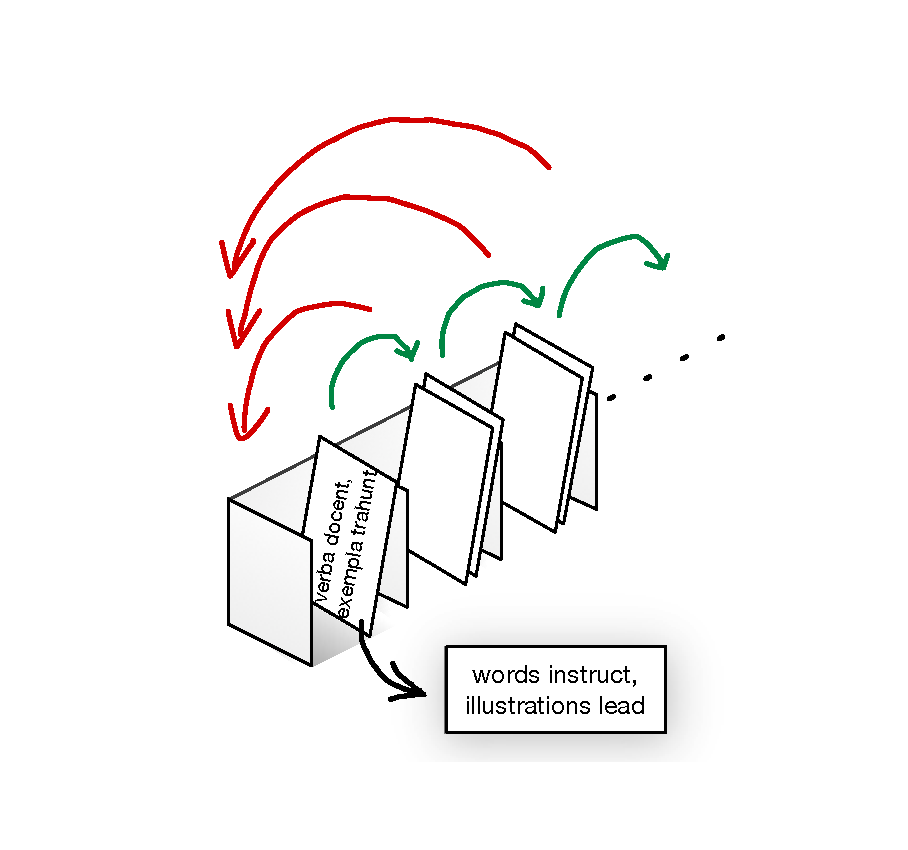
\includegraphics[width=0.4\textwidth]{membox_illustration.pdf}
	\caption{Possible \emph{concrete syntax} of a Leitner's Learning Box}
	\label{fig:membox_depiction}
\end{figure}
\FloatBarrier

For a more detailed overview, we recommend you read the introduction to Part II, Leitner's Learning Box. But for now, enough discussion! To get started, press
the new wizard button and navigate to ``Examples/eMoflon Handbook Examples/'' (Fig.).

% INCLUDE IMAGES AND INSTRUCTIONS ON HOW TO GET A 'JUMP' STARTED

Download the file set - visual or textual - that you'd like to learn about. Remember, there's no difference between the two syntaxes, this is purely a matter of
preference. Snoop around the files and to get familiar with what you'll be working with, then carry on to the next section to get started with SDMs.
